% ============================================================================
\section{Classical synthesis}
% ============================================================================

% --- Source: CMU Introduction to TTS (Works cited 6); TTS Lecture Material Generation Request ---
\begin{frame}{Pre-2016 Era: Corpus-Based and Concatenative Synthesis}
  \begin{itemize}
    \item Early systems used \textbf{unit selection}: recording lots of speech from a single speaker and splitting it into small parts (like diphones or syllables).
    \item During synthesis, an algorithm picks which units to use by balancing:
    \begin{itemize}
      \item \textbf{Target cost} (how well each piece matches the desired sound)
      \item \textbf{Join cost} (how smooth the pieces sound when joined together)
    \end{itemize}
    \item This gives good local naturalness, but is not very flexible and can sound glitchy if needed transitions are missing from the database.
  \end{itemize}
\end{frame}

% --- Source: CMU SPSS lecture (Works cited 7); Lecture-12 tts\_and\_vc ---
\begin{frame}{Statistical Parametric Synthesis}
  \begin{itemize}\footnotesize
    \item Statistical Parametric Speech Synthesis (SPSS) mainly used HMMs to model speech features instead of storing raw audio.
    \item SPSS models capture the spectral envelope, fundamental frequency ($F_0$), and duration of speech segments.
    \item Speaker adaptation is possible by updating a pre-trained model with a small amount of new speaker data, using MAP or linear regression techniques.
    \item Trajectory HMMs were introduced to make transitions between features smoother and output speech more natural.
  \end{itemize}
  \centering
  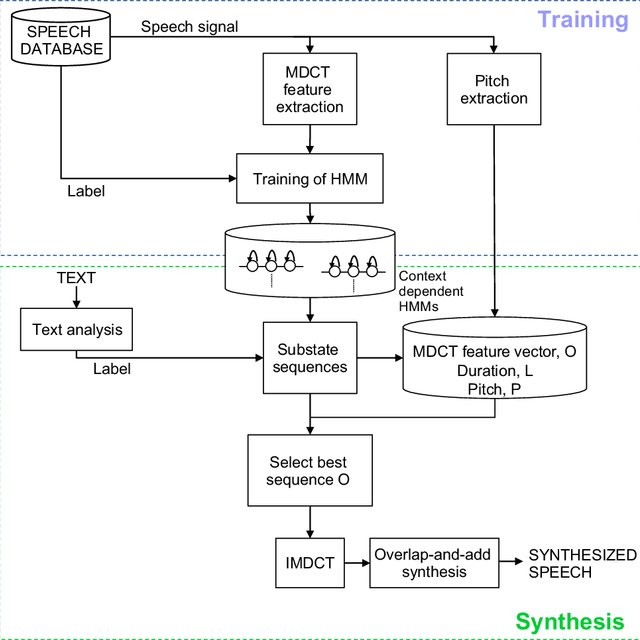
\includegraphics[width=\textwidth,height=0.55\textheight,keepaspectratio]{assets/New-Lecture-TTS/tts-hmm-based.png}
\end{frame}
